\documentclass[11pt,a4paper]{article}
\usepackage[T1]{fontenc}
\usepackage[utf8]{inputenc}
\usepackage{lmodern}
\usepackage[margin=22mm,headheight=14pt]{geometry}
\usepackage{amsmath,amssymb}
\usepackage{graphicx,xcolor}
\usepackage{array,longtable,booktabs,listings}
\usepackage{tikz,microtype,enumitem,needspace,titlesec,fancyhdr}
\usepackage{hyperref}
\definecolor{navy}{HTML}{18334D}
\definecolor{linkblue}{HTML}{176B91}
\definecolor{codebg}{HTML}{F2F5F7}
\hypersetup{colorlinks=true,linkcolor=linkblue,urlcolor=linkblue,
 pdftitle={Closed-loop CRIMSON netlist integration in Starfish},
 pdfsubject={Mathematics and proposed NumPy implementation},
 bookmarksnumbered=false,breaklinks=true}
\urlstyle{same}
\setcounter{secnumdepth}{0}
\setcounter{tocdepth}{1}
\setlength{\parindent}{0pt}
\setlength{\parskip}{6pt plus 1pt}
\setlength{\emergencystretch}{3em}
\sloppy
\allowdisplaybreaks[1]
\setlist{leftmargin=*,itemsep=3pt,topsep=4pt,parsep=2pt}
\titleformat{\section}{\Large\sffamily\bfseries\color{navy}}{}{0pt}{}
\titleformat{\subsection}{\large\sffamily\bfseries\color{navy}}{}{0pt}{}
\titlespacing*{\section}{0pt}{18pt}{8pt}
\titlespacing*{\subsection}{0pt}{12pt}{5pt}
\pagestyle{fancy}\fancyhf{}
\fancyhead[L]{\small\sffamily\color{navy}STARFISH / CRIMSON}
\fancyhead[R]{\small\sffamily Closed-loop implementation plan}
\fancyfoot[C]{\small\thepage}
\renewcommand{\headrulewidth}{.3pt}
\lstset{basicstyle=\ttfamily\footnotesize,breaklines=true,
 breakatwhitespace=false,columns=fullflexible,keepspaces=true,
 showstringspaces=false,backgroundcolor=\color{codebg},
 frame=single,rulecolor=\color{black!15},xleftmargin=5pt,xrightmargin=5pt,
 aboveskip=8pt,belowskip=8pt,upquote=true}
\begin{document}
\begin{titlepage}
\vspace*{28mm}
{\sffamily\color{navy}\Huge\bfseries Closed-loop CRIMSON\\[6pt]
netlist integration\\[6pt]in Starfish\par}
\vspace{12mm}
{\sffamily\Large Mathematics and proposed implementation\par}
\vspace{6mm}
{\large NumPy/reference backend\par}
\vspace{5mm}
20 October 2026
\vfill
\hrule\vspace{5mm}
\textbf{Planning document.} Source findings, proposed equations, software
interfaces, lifecycle changes and validation gates are identified explicitly.
This export does not implement the proposed runtime.
\vspace{5mm}
\end{titlepage}
\tableofcontents
\clearpage
\Needspace{6\baselineskip}
\section{1. Objective and status}
\textbf{Status: proposed implementation; no closed-loop Starfish runtime is introduced by this document.} Source review date: 2026-10-20.

The objective is to connect Starfish's 1D vessel network to a group of CRIMSON boundary circuits that share a downstream return circuit. The return circuit completes the circulation between the arterial outlets and the heart-side boundary. The implementation will use the \textbf{NumPy/reference} netlist-py backend selected through the existing root \texttt{netlist\_\allowbreak{}config.\allowbreak{}py}.

The expected result is a simulation in which vessel endpoint pressures and flows, upstream circuit states, and downstream return states satisfy one consistent boundary coupling calculation at each timestep. Controllers and valves advance once along the accepted state trajectory. Output includes the return circuit as well as the vessel and upstream circuit histories.

The work has three parts:


\begin{enumerate}
\item Reuse netlist-py's global circuit assembly and interface responses.


\item Introduce a coordinated characteristic boundary solve in Starfish.


\item Establish a C++ reference for the same physical model and coupling schedule.


\end{enumerate}
Existing C++ adapters, worker sources, bindings and integration call sites must remain available for reference. The previously disabled production C++ calls remain commented out. Production execution continues to use NumPy/reference.

\Needspace{6\baselineskip}
\section{2. Current capability and missing integration}
\Needspace{5\baselineskip}
\subsection{2.1 What is implemented in Starfish}
The current path is:


\begin{lstlisting}
Starfish Netlist boundary
  -> NetlistBoundaryInterface
  -> NetlistBoundaryManager
  -> NetlistPyAdapter
  -> independent reference boundary circuits
\end{lstlisting}
Each endpoint requests a scalar affine relation, solves its characteristic equation, and records its pressure and flow. The manager then supplies every surface's accepted input to the circuit update at the end of the timestep.

The current adapter explicitly rejects a nonempty \texttt{netlist\_\allowbreak{}closed\_\allowbreak{}loop\_\allowbreak{}downstream.\allowbreak{}xml}. The current characteristic interface also assumes zero flow when a port is blocked. It does not implement a general pressure-driven circuit port that returns nonzero flow.

The completed tutorial comparisons exercise independent boundary circuits. Feedback between a blood-loss observer and a heart controller does not, by itself, establish a closed hydraulic return path.

\Needspace{5\baselineskip}
\subsection{2.2 What is already available in netlist-py}
The reviewed checkout provides:


\begingroup\footnotesize
\setlength{\tabcolsep}{4pt}
\renewcommand{\arraystretch}{1.17}
\begin{longtable}{>{\raggedright\arraybackslash}p{\dimexpr0.36000\linewidth-2\tabcolsep\relax}>{\raggedright\arraybackslash}p{\dimexpr0.64000\linewidth-2\tabcolsep\relax}}
\toprule
\textbf{Existing capability} & \textbf{Relevant API/module} \\
\midrule
\endfirsthead
\textbf{Existing capability} & \textbf{Relevant API/module} \\
\midrule
\endhead
\bottomrule
\endfoot
Parse downstream circuits and their explicit connections & \texttt{Netlist\allowbreak{}Xml\allowbreak{}Reader.\allowbreak{}parse\_\allowbreak{}downstream\_\allowbreak{}netlist\_\allowbreak{}circuit\_\allowbreak{}with\_\allowbreak{}controls} \\[3pt]
Prepare one connected subsection and its initial runtime arrays & \texttt{Netlist\allowbreak{}Case.\allowbreak{}prepare\_\allowbreak{}closed\_\allowbreak{}loop\_\allowbreak{}subsection} \\[3pt]
Assemble rectangular local contributions and shared junction equations & \texttt{Closed\allowbreak{}Loop\allowbreak{}Downstream\allowbreak{}Subsection\_\allowbreak{}reference} \\[3pt]
Compute full pressure and flow responses between ports & \texttt{compute\_\allowbreak{}interface\_\allowbreak{}response}, \texttt{compute\_\allowbreak{}closed\_\allowbreak{}loop\_\allowbreak{}diode\_\allowbreak{}interface\_\allowbreak{}response} \\[3pt]
Accept histories and select next-step diode flags & \texttt{finalize\_\allowbreak{}closed\_\allowbreak{}loop\_\allowbreak{}diode\_\allowbreak{}timestep} \\[3pt]
Resolve owner-local controller observations and targets & Closed-loop observation layout and reference controller manifest APIs \\[3pt]
Run an upstream standalone closed-loop example & Closed-loop replacement driver and existing C++ oracle checks \\[3pt]
\end{longtable}
\endgroup
These capabilities support reuse of the circuit mathematics. They do not automatically integrate the Starfish characteristic boundary equations.

\Needspace{5\baselineskip}
\subsection{2.3 Coupling method proposed here}
\textbf{Use a simultaneous solve of the connected Starfish endpoint characteristic unknowns, with circuit state, controller targets and valve modes frozen during that solve.}

The upstream closed-loop 0D replacement driver preserves a delayed exchange with separate provisional and published port snapshots. This proposal defines a different external coupling method for the 1D vessel solver. Its global circuit equations can be checked against C++; its complete trajectory must be compared against a C++ circuit backend driven by the same Starfish schedule. Agreement with a native delayed 0D replacement trajectory is a separate claim.

\Needspace{6\baselineskip}
\section{3. Physical model, scope and inputs}
\Needspace{5\baselineskip}
\subsection{3.1 Circulation topology}

\begin{center}
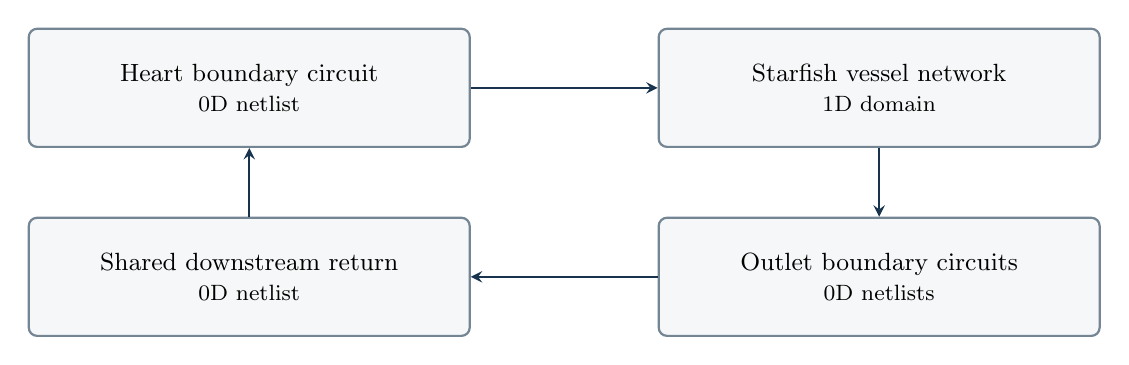
\begin{tikzpicture}[>=stealth,line width=.8pt,
 box/.style={draw=navy!60,rounded corners=3pt,fill=navy!4,
 minimum width=56mm,minimum height=15mm,align=center,font=\small}]
\node[box] (heart) at (0,0) {Heart boundary circuit\\\footnotesize 0D netlist};
\node[box] (vessels) at (8,0) {Starfish vessel network\\\footnotesize 1D domain};
\node[box] (outlets) at (8,-2.4) {Outlet boundary circuits\\\footnotesize 0D netlists};
\node[box] (return) at (0,-2.4) {Shared downstream return\\\footnotesize 0D netlist};
\draw[->,navy] (heart) -- (vessels);
\draw[->,navy] (vessels) -- (outlets);
\draw[->,navy] (outlets) -- (return);
\draw[->,navy] (return) -- (heart);
\end{tikzpicture}
\end{center}
The arrows indicate a typical physiological flow direction. Actual component flows remain signed and may reverse.

Starfish supplies the 1D vessel domain. A generated 0D replacement of those vessels is not required in the proposed production path. The upstream generated replacement remains useful as a separately validated reference experiment.

Closing an existing example requires an explicit return topology and its physical parameters. Independent prescribed-pressure outlet reservoirs cannot be assumed to become a return circuit merely by enabling a flag. Retain fixed reference nodes where the actual component formulation requires them; do not delete compliance reference nodes indiscriminately.

\Needspace{5\baselineskip}
\subsection{3.2 Initial supported scope}

\begin{itemize}
\item One downstream subsection with multiple attached upstream boundary circuits.


\item Explicit proximal and distal vessel endpoint bindings.


\item Physical surface ID 0, nonconsecutive surface IDs and reversed component orientation.


\item Constant timestep and \(\mathrm{alfi}=1\) for the first production milestone.


\item The reference implementation's supported R/C/L, volume and chamber equations.


\item Automatic diode modes and shared controller scheduling in a later milestone.


\item A case-defined source/sink ledger when hemorrhage or another external loss is present.


\end{itemize}
Additional independent boundary circuits may coexist once mixed scheduling is validated. Multiple downstream subsections require their own ownership and scheduling extension; they are outside the first milestone.

\Needspace{5\baselineskip}
\subsection{3.3 Case layout}

\begin{lstlisting}
case/
    input.xml
    netlist_surfaces.xml
    netlist_closed_loop_downstream.xml
    controller_reference.py             if declared
    controller.py                       retained C++ version, if available
    inflow.csv                          only if the physical case declares it
\end{lstlisting}
The downstream XML declares the upstream surface/node associated with each shared downstream node. A connection is identified by physical circuit and node identities, never by a guessed matrix offset.

\Needspace{6\baselineskip}
\section{4. Notation and units}

\begingroup\footnotesize
\setlength{\tabcolsep}{4pt}
\renewcommand{\arraystretch}{1.17}
\begin{longtable}{>{\raggedright\arraybackslash}p{\dimexpr0.19000\linewidth-2\tabcolsep\relax}>{\raggedright\arraybackslash}p{\dimexpr0.81000\linewidth-2\tabcolsep\relax}}
\toprule
\textbf{Symbol} & \textbf{Meaning} \\
\midrule
\endfirsthead
\textbf{Symbol} & \textbf{Meaning} \\
\midrule
\endhead
\bottomrule
\endfoot
\(n\), \(\Delta t\) & Accepted timestep index and physical timestep \\[3pt]
\(h^n\) & Accepted circuit histories retained at the start of the step \\[3pt]
\(\theta^n\) & Runtime R/C/L/E/V0 values and prescribed values used this step \\[3pt]
\(z^n\) & Retained diode flags; active interface modes are derived from them \\[3pt]
\(x\) & Global circuit solution vector, including current and history columns \\[3pt]
\(A_c\), \(f\) & Global circuit matrix and RHS contribution independent of external port inputs \\[3pt]
\(u\) & Vector of prescribed inputs to the netlist, one per external port \\[3pt]
\(p\), \(q\) & External port pressures and signed external flows \\[3pt]
\(P_v\), \(Q_v\) & Starfish pressure and axial flow at a vessel endpoint \\[3pt]
\(\sigma_i\) & Starfish \texttt{flow\allowbreak{}Sign}: \(q_i=\sigma_i Q_{v,i}\) \\[3pt]
\(\eta_i\) & Circuit component orientation: \(q_{\mathrm{component},i}=\eta_i q_i\) \\[3pt]
\(R_i\) & Starfish's local 2 by 2 characteristic-to-pressure/flow transform \\[3pt]
\(w_i\), \(k_i\) & Unknown incoming and known outgoing characteristic increments \\[3pt]
\(H_p\), \(H_q\) & Responses of port pressure and external flow to \(u\) \\[3pt]
\end{longtable}
\endgroup
For new Starfish physiological examples, use Pa, m\textsuperscript{3}/s, m\textsuperscript{3} and seconds. Then resistance has units Pa\ensuremath{\cdot}s/m\textsuperscript{3}, compliance m\textsuperscript{3}/Pa, inertance Pa\ensuremath{\cdot}s\textsuperscript{2}/m\textsuperscript{3}, and chamber elastance Pa/m\textsuperscript{3}. Archived upstream C++ fixtures retain their original consistent units and must be labelled accordingly.

The Starfish endpoint sign \(\sigma\) and the circuit orientation sign \(\eta\) have different responsibilities. The upstream response functions already account for their circuit orientation. Apply \(\sigma\) at the Starfish interface exactly once; do not apply \(\eta\) again to an already external-flow response.

\Needspace{6\baselineskip}
\section{5. Circuit equations and global assembly}
\Needspace{5\baselineskip}
\subsection{5.1 Component equations}
For component flow from start node \(s\) to end node \(e\), the resistor equation is


\nopagebreak[3]
\[
p_s-p_e-Rq=0.
\]


With effective increment \(\Delta t_e\), backward Euler gives the capacitor and inductor equations


\nopagebreak[3]
\[
p_s-p_e-p_s^n+p_e^n-\frac{\Delta t_e}{C}q=0,
\]



\nopagebreak[3]
\[
p_s-p_e-\frac{L}{\Delta t_e}q+\frac{L}{\Delta t_e}q^n=0.
\]


For the existing volume component convention,


\nopagebreak[3]
\[
V-\Delta t_e q-V^n=0.
\]


A pressure chamber additionally imposes the source's absolute start-node law


\nopagebreak[3]
\[
\frac{p_s}{E}-V=-V_0,
\qquad p_s=E(V-V_0).
\]


Preserve this implemented law when integrating the library. Replacing it with a different pressure-difference or transmural law would change the model. A plain volume tracker has no chamber E/V0 slots.

An open diode uses its resistive equation; a closed diode imposes \(q = 0\). Valve flags are fixed during each solve. Histories enter through explicit identity equations and are not reset from XML on every step.

\Needspace{5\baselineskip}
\subsection{5.2 Shared junction equations}
Keep the pressure unknowns belonging to each owner, then enforce equality at the shared physical junction:


\nopagebreak[3]
\[
p_{\mathrm{upstream},j}-p_{\mathrm{downstream},j}=0.
\]


The shared Kirchhoff conservation equation is


\nopagebreak[3]
\[
\sum_{\text{branches ending at }j}q
-\sum_{\text{branches starting at }j}q=0.
\]


Local KCL rows at deferred shared nodes are handled by the upstream layout builder. Keeping those rows and adding another independent junction equation would overconstrain the assembly. Use its canonical deferred-node maps.

\Needspace{5\baselineskip}
\subsection{5.3 Global matrix}
Let \(x\) concatenate the upstream circuit vectors and then the downstream vector. Each local block can be rectangular. In compact form:


\nopagebreak[3]
\[
A_c=
\begin{bmatrix}
\operatorname{blockdiag}(A_1,\ldots,A_m,A_d)\\
J_q\\
J_p
\end{bmatrix},
\qquad A_c x=f+B u.
\]


\(J_q\) contains shared KCL equations, \(J_p\) pressure equalities, and \(B\) inserts the active external prescriptions with the correct orientation signs. All histories, parameters, modes and the effective increment are held fixed when writing this affine system.

Necessary row count:


\nopagebreak[3]
\[
\sum_i r_i+N_{\mathrm{shared\ KCL}}+N_{\mathrm{pressure\ equalities}}
=\sum_i c_i.
\]


A square matrix alone does not prove the model is valid. Contradictory prescriptions, a missing pressure datum or an invalid closed-valve topology can still make it singular or inconsistent. The chosen pressure reference and initial stored volumes must be physically consistent; do not add an arbitrary ground as a numerical repair.

The upstream original heart fixture provides a useful assembly check:


\begingroup\footnotesize
\setlength{\tabcolsep}{4pt}
\renewcommand{\arraystretch}{1.17}
\begin{longtable}{>{\raggedright\arraybackslash}p{\dimexpr0.60000\linewidth-2\tabcolsep\relax}>{\raggedright\arraybackslash}p{\dimexpr0.20000\linewidth-2\tabcolsep\relax}>{\raggedright\arraybackslash}p{\dimexpr0.20000\linewidth-2\tabcolsep\relax}}
\toprule
\textbf{Contribution} & \textbf{Rows} & \textbf{Columns} \\
\midrule
\endfirsthead
\textbf{Contribution} & \textbf{Rows} & \textbf{Columns} \\
\midrule
\endhead
\bottomrule
\endfoot
Heart & 14 & 15 \\[3pt]
First outlet & 8 & 9 \\[3pt]
Second outlet & 8 & 9 \\[3pt]
Downstream return & 7 & 9 \\[3pt]
Shared KCL & 2 & --- \\[3pt]
Pressure equalities & 3 & --- \\[3pt]
Total & 42 & 42 \\[3pt]
\end{longtable}
\endgroup
This is an existing upstream fixture, not a proposed SI parameter set for the Starfish tutorial.

\Needspace{6\baselineskip}
\section{6. Interface responses}
\Needspace{5\baselineskip}
\subsection{6.1 Compute responses without accepting state}
Choose a finite baseline input vector \(u_*\) in the frozen modes. Solve


\nopagebreak[3]
\[
A_c x_*=f+B u_*,\qquad A_c Y=B.
\]


This uses a multiple-RHS solve; no explicit inverse is required. The upstream implementation constructs unit RHSs at \textbf{active prescription equation rows} and applies its input signs. A flow solution-column index is not an RHS-row index, particularly after a pressure-mode row permutation.

Let \(G_p\) select current port pressures and \(G_q\) select component flows. With \(S_\eta=\operatorname{diag}(\eta_i)\), external flow is \(q=S_\eta G_qx\). Thus


\nopagebreak[3]
\[
H_p=G_pY,\qquad H_q=S_\eta G_qY,
\]



\nopagebreak[3]
\[
p_0=G_px_*-H_pu_*,\qquad
q_0=S_\eta G_qx_*-H_qu_*.
\]


The resulting port relations are


\nopagebreak[3]
\[
\boxed{p=p_0+H_pu,\qquad q=q_0+H_qu.}
\]


The upstream APIs return the responses with their orientation transforms already included. These equations explain their meaning, not another layer of sign multiplication to add around those APIs.

\Needspace{5\baselineskip}
\subsection{6.2 All ports prescribed by flow}
When every port supplies external flow, \(u=q\), so


\nopagebreak[3]
\[
\boxed{p=p_0+H_pq.}
\]


Off-diagonal entries represent communication through the return circuit. For example, \((H_p)_{12}\) is the change of pressure at port 1 caused by a change of flow at port 2 with accepted state and active modes fixed.

\Needspace{5\baselineskip}
\subsection{6.3 Why the scalar Hop is conditional}
The C++ scalar coefficient for port \(i\) has the form


\nopagebreak[3]
\[
p_i=(H_p)_{ii}q_i+\mathrm{Hop}_i,
\]



\nopagebreak[3]
\[
\mathrm{Hop}_i=(p_0)_i+\sum_{j\ne i}(H_p)_{ij}(q_*)_j.
\]


Consequently, \(\mathrm{Hop}_i\) generally differs from \((p_0)_i\). A single sweep of independent endpoint solves using these conditional offsets freezes the other flows at a snapshot. It is a lagged approximation, not the simultaneous system derived below. Iterating it would require convergence and failure criteria.

The proposed first implementation uses the direct small endpoint system and retains conditional scalar getters only for reference checks.

\Needspace{6\baselineskip}
\section{7. Coupled Starfish characteristic equations}
\Needspace{5\baselineskip}
\subsection{7.0 Relation to the 1D vessel equations}
For orientation, a standard form of the incompressible 1D vessel equations is


\nopagebreak[3]
\[
\frac{\partial A}{\partial t}+\frac{\partial Q_v}{\partial z}=0,
\]



\nopagebreak[3]
\[
\frac{\partial Q_v}{\partial t}
+\frac{\partial}{\partial z}\left(\alpha_m\frac{Q_v^2}{A}\right)
+\frac{A}{\rho}\frac{\partial p}{\partial z}
=f_{\mathrm{friction}}+Ag_z,
\qquad p=\mathcal{P}(A,z).
\]


Here \(\alpha_m\) is the momentum-profile coefficient, not the netlist timestep parameter \texttt{alfi}. The configured wall law and fluid model determine the local wave speeds and characteristic transform. This notation describes the vessel model; this integration does not replace the existing field discretization or select a new wall law.

At a subcritical external endpoint, the vessel interior supplies one outgoing characteristic and the boundary condition determines the incoming one. The coupled circuit relation supplies those missing endpoint equations for the whole group. If a case leaves the one-incoming-characteristic regime, this boundary construction requires a separate characteristic-count review.

\Needspace{5\baselineskip}
\subsection{7.1 Endpoint packet}
The current Starfish boundary update satisfies


\nopagebreak[3]
\[
\begin{bmatrix}\Delta P_{v,i}\\\Delta Q_{v,i}\end{bmatrix}
=R_i\begin{bmatrix}\omega_{i,0}\\\omega_{i,1}\end{bmatrix}.
\]


At a proximal endpoint, index 0 is unknown and index 1 is known. At a distal endpoint, index 1 is unknown and index 0 is known. Let \(j\) denote the unknown column and \(l\) the known column. Define


\nopagebreak[3]
\[
a_i=P^n_{v,i}+(R_i)_{0l}k_i,\qquad b_i=(R_i)_{0j},
\]



\nopagebreak[3]
\[
c_i=\sigma_i\left(Q^n_{v,i}+(R_i)_{1l}k_i\right),
\qquad d_i=\sigma_i(R_i)_{1j}.
\]


Then, in external circuit-flow coordinates,


\nopagebreak[3]
\[
p_i=a_i+b_iw_i,\qquad q_i=c_i+d_iw_i.
\]


Stacking the endpoints gives


\nopagebreak[3]
\[
p=a+D_pw,\qquad q=c+D_qw,
\]


where \(D_p=\operatorname{diag}(b_i)\) and \(D_q=\operatorname{diag}(d_i)\).

\Needspace{5\baselineskip}
\subsection{7.2 Simultaneous flow-driven solve}
Substitute the characteristic relations into the circuit pressure response:


\nopagebreak[3]
\[
a+D_pw=p_0+H_p(c+D_qw).
\]


Therefore solve


\nopagebreak[3]
\[
\boxed{(D_p-H_pD_q)w=p_0+H_pc-a.}
\]


For \(m\) connected ports, this is an \(m\) by \(m\) dense system. Reconstruct all endpoint pressures and flows from the same solution \(w\). Reconstruct each two-entry characteristic vector with its original known component; preserve the existing boundary flow bookkeeping and vessel pressure-to-area law.

For one independent port this reduces exactly to the existing scalar Robin characteristic equation, including the proximal/distal column selection and Starfish \texttt{flow\allowbreak{}Sign}. That reduction is a required regression check.

\Needspace{5\baselineskip}
\subsection{7.3 Alternative flow-coordinate expression}
If every \(d_i\ne0\), define


\nopagebreak[3]
\[
Z_c=D_pD_q^{-1},\qquad g=a-Z_cc.
\]


Then \(p=g+Z_cq\), and


\nopagebreak[3]
\[
(Z_c-H_p)q=p_0-g.
\]


This is useful for analysis. The characteristic-unknown form avoids requiring division by each \(d_i\) and directly matches the current boundary API.

\Needspace{6\baselineskip}
\section{8. Mixed pressure and flow modes}
\Needspace{5\baselineskip}
\subsection{8.1 Mode convention}

\begingroup\footnotesize
\setlength{\tabcolsep}{4pt}
\renewcommand{\arraystretch}{1.17}
\begin{longtable}{>{\raggedright\arraybackslash}p{\dimexpr0.29000\linewidth-2\tabcolsep\relax}>{\raggedright\arraybackslash}p{\dimexpr0.30000\linewidth-2\tabcolsep\relax}>{\raggedright\arraybackslash}p{\dimexpr0.41000\linewidth-2\tabcolsep\relax}}
\toprule
\textbf{Port condition} & \textbf{Quantity prescribed to netlist} & \textbf{Conjugate quantity returned} \\
\midrule
\endfirsthead
\textbf{Port condition} & \textbf{Quantity prescribed to netlist} & \textbf{Conjugate quantity returned} \\
\midrule
\endhead
\bottomrule
\endfoot
Flow permitted & External flow & Pressure \\[3pt]
Pressure-driven mode & External pressure & External flow \\[3pt]
\end{longtable}
\endgroup
A closed diode may lead to a zero-flow condition, but a general pressure-driven port need not return zero flow. Use its actual response.

Let \(F\) be a diagonal selector with entry 1 for a flow-input port and 0 for a pressure-input port. Let \(T=I-F\). Then


\nopagebreak[3]
\[
u=Fq+Tp.
\]


This vector has a declared quantity and unit per position. It is not a uniform flow vector, and \(H_p\) is not uniformly a resistance matrix in this case.

Substituting the characteristic relations gives


\nopagebreak[3]
\[
u=u_c+D_uw,\qquad u_c=Fc+Ta,\qquad D_u=FD_q+TD_p.
\]


\Needspace{22\baselineskip}
\subsection{8.2 Enforce the returned quantity at every endpoint}
At flow-input ports enforce the returned pressure; at pressure-input ports enforce the returned flow:


\nopagebreak[3]
\[
F\left[p-p_0-H_pu\right]
+T\left[q-q_0-H_qu\right]=0.
\]


The simultaneous boundary system is


\nopagebreak[3]
\[
\boxed{K_w w=r_w.}
\]



\nopagebreak[3]
\[
K_w=F(D_p-H_pD_u)+T(D_q-H_qD_u),
\]



\nopagebreak[3]
\[
r_w=F(p_0+H_pu_c-a)+T(q_0+H_qu_c-c).
\]


Setting \(F = I\) recovers the all-flow system. A genuinely blocked port with identically zero returned flow gives the expected zero-flow characteristic condition. This handles that special case without assuming every pressure mode is blocked.

\Needspace{5\baselineskip}
\subsection{8.3 Independent monolithic equation check}
For validation, the same endpoint result can be obtained without eliminating the circuit unknowns:


\nopagebreak[3]
\[
\begin{bmatrix}
A_c & -BD_u\\
FG_p+TG_q^{ext} & -(FD_p+TD_q)
\end{bmatrix}
\begin{bmatrix}x\\w\end{bmatrix}
=
\begin{bmatrix}
f+Bu_c\\Fa+Tc
\end{bmatrix},
\]


where \(G_q^{ext}=S_\eta G_q\). Compare this direct system against the response-based endpoint solve on small fixtures. It provides an independent check of elimination, signs, offsets and mixed-mode selection.

\Needspace{5\baselineskip}
\subsection{8.4 Scaling and conditioning}
Mixed rows constrain pressures or flows, and characteristic normalization can also vary. Use explicit positive row and unknown scales:


\nopagebreak[3]
\[
(W_rK_wW_c)y=W_rr_w,\qquad w=W_cy.
\]


Scaling changes numerical representation, not the physical equations. Record the selected physical scales, scaled residual and condition estimate. Reject singular or nonfinite solves. Do not repair them by adding diagonal leakage, clamping pressures, changing R/C/L values or dropping junction equations.

\clearpage
\Needspace{6\baselineskip}
\section{9. Worked analytical example}
Use a two-port resistive fixture in internally consistent arbitrary units: proximal resistances 2 and 4, a shared distal resistance 8, and reservoir pressure 3. This is an analytical coupling fixture, not a complete heart model.

The common pressure and port pressures are


\nopagebreak[3]
\[
p_d=3+8(q_1+q_2),\quad p_1=p_d+2q_1,\quad p_2=p_d+4q_2.
\]


Thus


\nopagebreak[3]
\[
H_p=\begin{bmatrix}10&8\\8&12\end{bmatrix},\qquad
p_0=\begin{bmatrix}3\\3\end{bmatrix}.
\]


At prescribed flows \((1, 2)\), pressures are \((29, 35)\). The conditional scalar pairs are \((\mathrm{dp\_dq},\mathrm{Hop})=(10,19)\) and \((12, 11)\). This immediately exposes confusion between the vector offset and the conditional Hop.

Now give the vessel characteristics


\nopagebreak[3]
\[
p_1=29-q_1,\qquad p_2=35-2q_2.
\]


The coupled endpoint equations become


\nopagebreak[3]
\[
\begin{bmatrix}11&8\\8&14\end{bmatrix}
\begin{bmatrix}q_1\\q_2\end{bmatrix}
=\begin{bmatrix}26\\32\end{bmatrix}.
\]


Their exact solution is


\nopagebreak[3]
\[
q_1=1.2,\quad q_2=1.6,\quad p_d=25.4,
\quad p_1=27.8,\quad p_2=31.8.
\]


Required checks include these values, both off-diagonal responses, invariance under a consistent port permutation, and equivalence to the monolithic solve.

\Needspace{6\baselineskip}
\section{10. Timestep, valve and controller lifecycle}
\Needspace{5\baselineskip}
\subsection{10.1 Accepted state}
Retain an explicit accepted state containing:


\begin{lstlisting}
accepted timestep index
accepted circuit histories
published current pressure/flow/volume observations
diode flags
controller state
runtime target arrays
last accepted external port pressure/flow vectors
\end{lstlisting}
A coefficient probe or endpoint trial must not change this state. In the reference path, protect accepted arrays from mutation through shared views.

\Needspace{5\baselineskip}
\subsection{10.2 Proposed Starfish schedule}
For the initial \(\mathrm{alfi}=1\) profile:


\begin{enumerate}
\item Retain \(h^n\), \(\theta^n\), controller state and diode flags.


\item Derive local interface reachability/modes from the retained valve flags.


\item Gather every connected vessel's characteristic packet from timestep \(n\).


\item Assemble the full-dt subsection and compute its port response at fixed state.


\item Solve the simultaneous characteristic system for all connected endpoints.


\item Solve the circuit at the resulting active port inputs with full \(\Delta t\). Check that its returned conjugate quantities match the endpoint solution.


\item Validate all proposed endpoint pressures, flows and areas, then scatter the endpoint values into Starfish's timestep \(n+1\) storage.


\item Run the existing vessel/interior and connection operations in their audited order. Retain the circuit candidate without accepting it during these calls.


\item After all required operations succeed, publish physical circuit values and accept circuit histories once. Determine next-step diode flags.


\item Update one shared controller schedule from the accepted physical observations and prepare targets for the following timestep.


\item Publish accepted output before runtime memory advances or flushes that step.


\end{enumerate}
The last point requires an explicit scheduling seam: network output and runtime memory management are currently entries in \texttt{numerical\allowbreak{}Objects}. Separate their publication/rollover role from the numerical phase so they cannot run ahead of closed-loop finalization. Preserve existing independent-case behavior.

All endpoint solves use one frozen packet set. A later endpoint cannot see an earlier endpoint's newly accepted circuit history. Do not advance a controller again during unit-response calculation or final circuit reassembly.

\Needspace{5\baselineskip}
\subsection{10.3 Valve behavior}
Reuse the source's local reachability and next-step diode predicate:


\nopagebreak[3]
\[
\mathrm{open}^{n+1}=
(p_s-p_e\ge-10^{-8})\;\lor\;(q\ge10^{-8}).
\]


These are literal legacy predicate thresholds in the case's units. They are not the proposed trajectory comparison tolerances. Preserve the kernel's published-state and history acceptance sequence.

Do not introduce same-step valve iteration as part of boundary coupling. The boundary system is simultaneous at fixed active valve flags; next-step mode selection remains a separate operation. Upstream reachability is local to each boundary circuit, not a walk through the whole return network.

\Needspace{5\baselineskip}
\subsection{10.4 Controller phase and ownership}
The existing Starfish adapter updates controllers after circuit acceptance. Retain that phase for the proposed first Starfish closed-loop profile and implement the same phase in its C++ comparison harness.

The upstream \texttt{controlled\_\allowbreak{}closed\_\allowbreak{}loop\_\allowbreak{}iter\_\allowbreak{}init} updates controllers before the solve using old published observations. Calling that driver entry point directly would change the Starfish schedule. Reuse lower-level assembly, observation and controller APIs with explicit orchestration instead.

Use one schedule spanning upstream and downstream owners:


\begin{itemize}
\item Gather physical current pressure/flow/volume columns for the correct owner.


\item Execute modern Python controllers by ascending priority.


\item Start each controller update with a fresh broadcast dictionary.


\item Expose only earlier controllers' broadcasts and merge with first-writer-wins semantics.


\item Execute the supported built-in group in its documented order.


\item Apply targets to explicit owner/kind/physical-ID/runtime-slot bindings.


\end{itemize}
Initialize built-in targets at time zero according to their source semantics. Setup validation must discard sampled updates and must not advance physical time or retained controller state. Conflicting destinations are rejected until an explicit ordered-write contract is implemented.

\Needspace{5\baselineskip}
\subsection{10.5 Failure handling and alpha}
A failed probe, missing endpoint, stale packet or incomplete circuit candidate must not accept history or increment counters. Prepare reference-side next state and controller results before retaining a successful transition where the APIs permit this. A failure after an external C++ harness has committed state must mark the run failed; do not promise rollback or retry it as though the old state were still current.

First implement and validate \(\mathrm{alfi}=1\). A future alpha-stage extension must define how Starfish supplies stage-compatible characteristics and endpoint states. Independent \(\alpha\Delta t\) probes, full-dt updates and the upstream replacement driver's first-query cache semantics are different contracts. Do not infer generalized-alpha support from the presence of an \texttt{alfi} argument.

\Needspace{6\baselineskip}
\section{11. Proposed software architecture}
\Needspace{5\baselineskip}
\subsection{11.1 Responsibilities and files}
The following names for new modules and APIs are proposals.


\begingroup\footnotesize
\setlength{\tabcolsep}{4pt}
\renewcommand{\arraystretch}{1.17}
\begin{longtable}{>{\raggedright\arraybackslash}p{\dimexpr0.36000\linewidth-2\tabcolsep\relax}>{\raggedright\arraybackslash}p{\dimexpr0.64000\linewidth-2\tabcolsep\relax}}
\toprule
\textbf{File} & \textbf{Proposed responsibility} \\
\midrule
\endfirsthead
\textbf{File} & \textbf{Proposed responsibility} \\
\midrule
\endhead
\bottomrule
\endfoot
\texttt{netlist\_\allowbreak{}config.\allowbreak{}py} & Keep the existing netlist-py location and reference backend policy \\[3pt]
\texttt{Utility\allowbreak{}Lib/\allowbreak{}netlist\allowbreak{}Closed\allowbreak{}Loop\allowbreak{}Py\allowbreak{}Adapter.\allowbreak{}py} (new) & Parse/setup one subsection; own accepted circuit state, response queries, candidates, controllers and downstream histories \\[3pt]
\texttt{Network\allowbreak{}Lib/\allowbreak{}netlist\allowbreak{}Coupling.\allowbreak{}py} (new) & Pure NumPy characteristic packet algebra, all-flow/mixed endpoint systems, reconstruction and residual checks \\[3pt]
\texttt{Network\allowbreak{}Lib/\allowbreak{}netlist\allowbreak{}Manager.\allowbreak{}py} & Explicit bindings, topology-based adapter selection, group coordination and one finalization \\[3pt]
\texttt{Network\allowbreak{}Lib/\allowbreak{}netlist\allowbreak{}Interface.\allowbreak{}py} & Preserve scalar path; expose packet/reconstruction helpers for grouped endpoints \\[3pt]
\texttt{Solver\allowbreak{}Lib/\allowbreak{}class\allowbreak{}Boundarys.\allowbreak{}py} & Separate preparation, validation and application of a boundary result \\[3pt]
\texttt{Solver\allowbreak{}Lib/\allowbreak{}class1Dflow\allowbreak{}Solver.\allowbreak{}py} & Insert the group operation and separate numerical stepping from output/memory rollover \\[3pt]
\texttt{Network\allowbreak{}Lib/\allowbreak{}class\allowbreak{}Vascular\allowbreak{}Network.\allowbreak{}py} & Audit initialization paths that currently assume independent terminal resistance \\[3pt]
\texttt{Unit\allowbreak{}Testing/\allowbreak{}} & Analytical, lifecycle, integration and backend comparison checks added during implementation \\[3pt]
New C++ validation sources under \texttt{ext/\allowbreak{}} & Closed-loop reference harness alongside the preserved existing worker \\[3pt]
\end{longtable}
\endgroup
The current \texttt{Netlist\allowbreak{}Py\allowbreak{}Adapter} remains the independent-circuit path. Adapter selection is based on validated topology, not a user-selectable production backend. A malformed downstream file raises an error rather than silently selecting independent circuits.

\Needspace{5\baselineskip}
\subsection{11.2 Proposed data contracts}

\begin{lstlisting}[language=Python]
# Schematic records: field names describe the contract, not implemented APIs.
PortBinding(
    physical_surface_id, vessel_id, endpoint_position, flow_sign,
    xml_circuit_index, internal_surface_id, port_position,
)

CharacteristicPacket(
    binding, timestep, memory_generation, dt,
    current_pressure, current_axial_flow, current_area,
    characteristic_matrix, known_increment,
    unknown_column, known_column,
)

PortResponse(
    source_state_version, timestep, effective_dt, active_modes, flow_input_mask,
    pressure_response, flow_response, pressure_offset, flow_offset,
)

BoundaryCandidate(
    source_state_version, port_order, active_inputs,
    pressures, external_flows, characteristic_increments,
    circuit_candidate, residuals,
)
\end{lstlisting}
Packets must own copies of any matrices or arrays that the system-equation object reuses. This matters when both ends of one vessel are in the group. The candidate must carry enough source-state identity to reject stale probes. The response's Boolean \texttt{flow\_\allowbreak{}input\_\allowbreak{}mask} is derived from, and validated against, its active modes. It is not an independent caller-selected mode override.

\Needspace{5\baselineskip}
\subsection{11.3 Proposed adapter operations}

\begin{lstlisting}[language=Python]
load(bindings, dt, case_directory)
begin_step(timestep, time, dt)
probe_port_response(flow_snapshot, pressure_snapshot)
solve_trial(active_inputs)
prepare_acceptance(boundary_candidate)
finalize_prepared_step(prepared_transition)
close()
\end{lstlisting}
\texttt{probe\_\allowbreak{}port\_\allowbreak{}response} and \texttt{solve\_\allowbreak{}trial} are observational with respect to accepted state. The adapter derives modes from its retained circuit state; callers cannot invent a contradictory mode vector. \texttt{prepare\_\allowbreak{}acceptance} validates complete endpoint coverage, timestep identity, physical publication, history and controller transitions. Finalization retains one completed step.

Freeze the mapping and group membership before stepping. Logging and output use physical identities; internal positive IDs remain implementation details.

\Needspace{5\baselineskip}
\subsection{11.4 Boundary algebra pseudocode}
The following sketch implements the equations in sections 7--8. Helpers, records, scaling selection and error handling are proposed interfaces.


\begin{lstlisting}[language=Python]
def solve_group(packets, response, physical_scales):
    # Each packet is frozen at the same timestep and memory generation.
    a, b, c, d = characteristic_coefficients(packets)
    Dp, Dq = np.diag(b), np.diag(d)
    F = np.diag(response.flow_input_mask.astype(np.float64))
    T = np.eye(len(packets)) - F

    Hp = response.pressure_response
    Hq = response.flow_response
    p0 = response.pressure_offset
    q0 = response.flow_offset

    uc = F @ c + T @ a
    Du = F @ Dq + T @ Dp
    matrix = F @ (Dp - Hp @ Du) + T @ (Dq - Hq @ Du)
    rhs = F @ (p0 + Hp @ uc - a) + T @ (q0 + Hq @ uc - c)
    w = solve_scaled_system(matrix, rhs, physical_scales)

    pressure = a + Dp @ w
    external_flow = c + Dq @ w
    active_inputs = F @ external_flow + T @ pressure
    check_response_residuals(pressure, external_flow, active_inputs, response)
    return reconstruct_boundary_candidate(packets, w, active_inputs)
\end{lstlisting}
The group coordinator next calls the circuit adapter's full-dt \texttt{solve\_\allowbreak{}trial} using these inputs and validates its actual physical publication before applying endpoint values. Neither this algebra nor that trial accepts state. Acceptance occurs at the explicit finalization seam after the numerical phase succeeds. The reconstruction helper retains physical flow signs, both known and unknown characteristic entries, and each boundary's existing bookkeeping.

\Needspace{6\baselineskip}
\section{12. Scheduling and boundary refactoring}
\Needspace{5\baselineskip}
\subsection{12.1 Existing dependency}
The current numerical object list interleaves the root boundary, vessel fields, connections and terminal boundaries. A boundary call both calculates its characteristic input and writes endpoint arrays immediately. Group coupling requires gathering all connected endpoint packets before applying their results.

Moving callbacks without auditing array access would risk mixing timestep \(n\) and \(n+1\) data. Runtime memory rollover is another dependency: array index \texttt{nmem} is not always the global timestep number.

\Needspace{5\baselineskip}
\subsection{12.2 Refactoring sequence}

\begin{enumerate}
\item Extract a preparation operation that computes the exact existing \texttt{update\allowbreak{}LARL} inputs and known characteristic from current timestep arrays.


\item Extract validation/application of \(\Delta P\), \(\Delta Q\), area and blood-flow bookkeeping.


\item Keep the ordinary boundary call as preparation \ensuremath{\rightarrow} scalar solve \ensuremath{\rightarrow} application. Establish equivalence for existing cases before adding grouping.


\item Add a grouped boundary object that gathers packets, solves once, validates every result and applies each member exactly once.


\item Schedule that group before any operation consuming its next-step endpoints. The reviewed field implementations read timestep \(n\) and write interior timestep \(n+1\) cells; confirm this for every activated solver variant.


\item Replace only the grouped members' individual scheduled calls. Preserve other field, connection and native-boundary ordering where compatible.


\item Finalize the netlist after the numerical phase succeeds, before accepted output and memory rollover. Audit normal and cycle execution paths.


\end{enumerate}
For the initial supported scheme, gather all group packets from timestep \(n\) and place the group before field advancement. If another scheme needs predicted data, introduce an explicit stage interface before enabling it.

The first milestone must either support a given alternate execution path or reject it at setup with a specific reason. A second hidden, unsynchronized boundary update in cycle mode is not acceptable.

\Needspace{6\baselineskip}
\section{13. Identity mapping and initialization}
\Needspace{5\baselineskip}
\subsection{13.1 Physical surface 0}
The current Starfish adapter accepts surface 0. The reviewed upstream downstream parser and subsection setup require positive surface IDs.

Use an explicit bijection, for example:


\begingroup\footnotesize
\setlength{\tabcolsep}{4pt}
\renewcommand{\arraystretch}{1.17}
\begin{longtable}{>{\raggedright\arraybackslash}p{\dimexpr0.23000\linewidth-2\tabcolsep\relax}>{\raggedright\arraybackslash}p{\dimexpr0.23000\linewidth-2\tabcolsep\relax}>{\raggedright\arraybackslash}p{\dimexpr0.30000\linewidth-2\tabcolsep\relax}>{\raggedright\arraybackslash}p{\dimexpr0.24000\linewidth-2\tabcolsep\relax}}
\toprule
\textbf{Physical surface} & \textbf{XML circuit index} & \textbf{Internal positive surface} & \textbf{Port position} \\
\midrule
\endfirsthead
\textbf{Physical surface} & \textbf{XML circuit index} & \textbf{Internal positive surface} & \textbf{Port position} \\
\midrule
\endhead
\bottomrule
\endfoot
0 & 1 & 1 & 0 \\[3pt]
4 & 2 & 2 & 1 \\[3pt]
12 & 3 & 3 & 2 \\[3pt]
\end{longtable}
\endgroup
This example preserves the existing sorted-surface-to-XML mapping, then records every association. Runtime code gathers and scatters using that table; it must not independently sort vessels, circuits or return connections.

Because the upstream parser reads paths and validates connection surface IDs, normalize downstream surface references in a private XML copy before calling it. Rewrite only the mapped upstream surface IDs. Preserve node IDs, circuit indices, physical parameters, declaration order and original XML files. Reject connections to unknown surfaces.

Persist original and normalized XML with the mapping and their hashes. Resolve controller modules through an explicit original/snapshotted case directory; normalizing XML in another directory must not change script discovery. Owner labels and output filenames are translated back to physical identities.

\Needspace{5\baselineskip}
\subsection{13.2 Vessel and circuit initialization}
Current network initialization includes cumulative terminal resistance and proximal-Netlist heuristics. A shared downstream circuit changes those assumptions. Reusing independent-terminal resistance splitting could produce inconsistent initial flows even when the timestep equations are correct.

For the first fixture, use an explicitly documented initial pressure/flow profile and matching circuit histories/volumes. Audit the existing \texttt{Constant\allowbreak{}Pressure} path and its remaining resistance-dependent setup before using it. Reject incompatible automatic initialization rather than silently applying an open-terminal estimate.

Document any intentional initial pressure jump and its resulting startup transient. Do not reset chamber volume to eliminate a transient after a run has started. A future equilibrium initializer can solve the coupled steady equations with the same constraints and a stated heart phase; it is a separate feature from a functioning timestep coupling.

The existing boundary callback rejects negative calculated vessel pressure. The initial supported case must fit that pressure convention. A physiological model needing negative gauge pressures requires an explicit review of the vessel wall law and pressure checks; the closed-loop adapter must not hide it by clipping or shifting pressures independently of the circuit.

\Needspace{6\baselineskip}
\section{14. C++ reference and comparison strategy}
\Needspace{5\baselineskip}
\subsection{14.1 Current worker limitation}
The retained \texttt{Crimson\allowbreak{}Netlist\allowbreak{}Runtime:\allowbreak{}:\allowbreak{}create\allowbreak{}Surface} creates independent \texttt{Netlist\allowbreak{}Circuit} instances. It does not build the shared downstream subsection. Merely running that worker next to a downstream XML file would not provide a closed-loop C++ reference.

Add separate validation code that uses the source's \texttt{Netlist\allowbreak{}Boundary\allowbreak{}Circuit\allowbreak{}When\allowbreak{}Downstream\allowbreak{}Circuits\allowbreak{}Exist}, \texttt{Netlist\allowbreak{}Closed\allowbreak{}Loop\allowbreak{}Downstream\allowbreak{}Circuit} and \texttt{Closed\allowbreak{}Loop\allowbreak{}Downstream\allowbreak{}Subsection} responsibilities. Review their ownership and initialization APIs before designing the harness. Preserve the current worker and its behavior.

\Needspace{5\baselineskip}
\subsection{14.2 Three levels of comparison}
\textbf{A. Circuit equation and prescribed-port comparison.} Supply identical explicit pressure/flow vectors, parameters, timestep, histories and modes to the C++ and NumPy subsections. Compare assembled equations, current solutions, conditional scalar getters and accepted trajectories. Frozen-state unit responses must not accidentally advance or reuse a stale C++ cached solve. Where necessary, expose native assembled matrices or an explicit cache-reset validation seam. A NumPy calculation labelled as C++ output is not evidence.

\textbf{B. Same Starfish coupling algorithm, different circuit backend.} Drive the proposed simultaneous endpoint solver with each backend's independently computed response. Both runs own their own state, controllers and trajectories. Use the same post-acceptance controller phase and output sampling. This is the required full Starfish C++ versus NumPy integration comparison.

\textbf{C. Native upstream delayed replacement trajectory.} Retain the existing upstream original-heart/BCT oracle checks as evidence for that profile. They use a generated 0D domain and its source exchange schedule. Differences between that model and a 1D Starfish vessel domain are not backend errors.

Levels A and B are required for this integration. Existing level C evidence does not replace either one.

\Needspace{6\baselineskip}
\section{15. Validation requirements}
This section specifies future implementation checks. No new tests or solver runs were performed to author this planning document.

\Needspace{5\baselineskip}
\subsection{15.1 Analytical and algebraic gates}

\begin{itemize}
\item The two-port example in section 9, including conditional Hop values.


\item One-port and diagonal-response reduction to the existing scalar solver.


\item Mixed pressure/flow reduction, including nonzero returned flow.


\item Response elimination versus the independently assembled monolithic system.


\item Explicit surface 0 and nonconsecutive surface mappings.


\item Proximal/distal bindings and reversed circuit component orientation.


\item Invariance under consistent permutations of port order and declaration order.


\item Shared KCL, pressure equality and block row/column count checks.


\item Diagnostic failures for singular topology and contradictory prescriptions.


\end{itemize}
Check the global linear backward error in scaled coordinates:


\nopagebreak[3]
\[
\rho_A=\frac{\|A_cx-b\|_\infty}
{\|A_c\|_\infty\|x\|_\infty+\|b\|_\infty}.
\]


Handle an exactly zero denominator explicitly. Apply the same form to the endpoint system. Because equation rows have different units, use stated row and variable scaling before forming a norm across the whole matrix. Also report physical-unit residuals for individual KCL and equality constraints.

\Needspace{5\baselineskip}
\subsection{15.2 Lifecycle gates}

\begin{itemize}
\item Repeated probes leave histories, flags, targets and controller counters unchanged.


\item Exactly one state for every connected endpoint is required for acceptance.


\item Duplicate, stale, nonfinite and cross-timestep packets are rejected.


\item New histories come from current published columns, not old-history columns.


\item Downstream and upstream histories advance together.


\item Closed/open diode flags and interface mode sequences match the reference.


\item Owner-local observations and cross-owner progressive broadcasts are correct.


\item Controller setup samples do not become runtime updates.


\item Both ends of one vessel work without shared-matrix view corruption.


\item Memory rollover, output cadence and cleanup preserve step/row alignment.


\item An incomplete failed timestep adds no accepted output row.


\end{itemize}
\Needspace{5\baselineskip}
\subsection{15.3 Physical conservation}
At each shared junction report


\nopagebreak[3]
\[
r_{q,j}=\sum q_{\mathrm{ending}}-\sum q_{\mathrm{starting}},
\qquad r_{p,j}=p_{\mathrm{upstream},j}-p_{\mathrm{downstream},j}.
\]


For the 1D domain, compute vessel volume from the declared spatial quadrature of \(A\). For a declared closed system with no physical source or loss,


\nopagebreak[3]
\[
V_{\mathrm{total}}^{n+1}-V_{\mathrm{total}}^n
=\epsilon_{\mathrm{discretization}}.
\]


For an explicitly declared loss/source model, use


\nopagebreak[3]
\[
\Delta V_{\mathrm{total}}
=\int_{t_n}^{t_{n+1}}(Q_{\mathrm{source}}-Q_{\mathrm{loss}})\,dt
+\epsilon_{\mathrm{discretization}}.
\]


Construct the 0D storage ledger from the actual model: chamber volumes and declared compliance storage must be counted once. An electrical reference node is not automatically an external blood-loss outlet. Do not infer a loss from every grounded component.

Starfish's vessel discretization need not conserve the quadrature-derived volume to machine precision. Report the defect and verify its resolution dependence; distinguish it from an algebraic shared-junction residual.

\Needspace{5\baselineskip}
\subsection{15.4 Trajectory comparisons and tolerances}
Compare every accepted upstream/downstream pressure, flow and volume column, every saved vessel P/Q/A dataset, time arrays, step counts and mode sequence. Record controller outputs/state diagnostics at an identical phase.

For SI cases, the current independent-backend thresholds are a starting proposal: \(\mathrm{rtol}=5\times10^{-11}\), pressure \(\mathrm{atol}=10^{-8}\,\mathrm{Pa}\), flow \(10^{-12}\,\mathrm{m}^3/\mathrm{s}\), volume \(10^{-12}\,\mathrm{m}^3\), and area \(10^{-14}\,\mathrm{m}^2\). These thresholds have not been demonstrated for the proposed Starfish closed-loop integration.

Retain the upstream original-unit fixture's reviewed error budget when using its archived evidence. Do not relabel native-unit errors as SI errors or relax thresholds simply to obtain a pass. If a gate fails, identify the first divergent equation, history, controller update or valve event before reviewing whether its numerical budget is appropriate.

Use timestep refinement with the same underlying physical input/controller law and compare event times in physical time. Existing 0.5-second upstream evidence is not a long-duration settling result. Longer physiological and hemorrhage runs belong after the short deterministic gates pass.

The vessel CFL restriction remains necessary, but it alone does not establish stability of the combined circuit, wall and controller system. Exercise stiff return compliances, high resistance contrasts and the documented control gains at several timestep sizes. Backward Euler circuit history is first order; the second-order form of an interior MacCormack update does not, by itself, make the complete coupled trajectory second order. Report observed convergence rather than assigning an order from one subsystem's scheme name.

\Needspace{5\baselineskip}
\subsection{15.5 Required fixtures}

\begingroup\footnotesize
\setlength{\tabcolsep}{4pt}
\renewcommand{\arraystretch}{1.17}
\begin{longtable}{>{\raggedright\arraybackslash}p{\dimexpr0.36000\linewidth-2\tabcolsep\relax}>{\raggedright\arraybackslash}p{\dimexpr0.64000\linewidth-2\tabcolsep\relax}}
\toprule
\textbf{Fixture} & \textbf{Main purpose} \\
\midrule
\endfirsthead
\textbf{Fixture} & \textbf{Main purpose} \\
\midrule
\endhead
\bottomrule
\endfoot
Two-port passive shared resistance & Off-diagonal response and exact endpoint solve \\[3pt]
Shared RC return & History carry and reservoir storage \\[3pt]
R/L/volume variant & Flow history and volume-column ownership \\[3pt]
Surface 0, nonconsecutive IDs, reversed interface & Identity and orientation \\[3pt]
One pressure-input port with nonzero returned flow & General mixed-mode boundary equation \\[3pt]
Original upstream heart/return fixture & Native C++ assembly, getters and carried state \\[3pt]
Small explicit Starfish vessel/return case & End-to-end simultaneous coupling \\[3pt]
Heart/valve case & Valve events and chamber publication \\[3pt]
Downstream observer and upstream feedback & Global controller schedule and ownership \\[3pt]
Closed circulation with declared bleed & Total-volume loss ledger \\[3pt]
\end{longtable}
\endgroup
Repeat the existing independent-circuit and tutorial comparisons as regression gates during implementation. Their previous success does not prove new closed-loop behavior.

\Needspace{6\baselineskip}
\section{16. Results, provenance and timing}
Follow the existing per-case comparison layout, with separate backend output directories and a fresh numbered directory for each execution:


\begin{lstlisting}
case/results_netlist_comparison/main_001/
    comparison.md
    comparison.json
    cpp/
        inputs/                         original and normalized inputs
        run.json
        console.log
        SolutionData_001/
    python/
        inputs/
        run.json
        console.log
        SolutionData_001/
\end{lstlisting}
Add downstream files using a documented index convention. The source's first downstream XML circuit is 1-based, while its history label is typically \texttt{downstream\allowbreak{}Circuit\_\allowbreak{}0}. Record that mapping explicitly rather than guessing from the filename. Physical surface 0 remains \texttt{surface\_\allowbreak{}0}.

Save bindings, port order, normalization hashes, case units, controller phase, backend/code identity, dt/alpha, physical scales, accepted counts and validation thresholds. Preserve originals and existing results.

Report initialization, complete solve, circuit assembly/response work, endpoint solve, controller work, output and whole-process time. Use sequential fresh processes with the same thread settings. Label single-run observations and any diagnostic-I/O differences. Matrix snapshots or detailed per-step traces should be optional diagnostics, not always-on benchmark overhead.

First use clear dense solves. Reuse a factorization only after correctness is established, with an invalidation key covering accepted state dependencies, effective dt, topology, active mode rows and runtime parameter changes. RHS changes and matrix changes have different reuse requirements. Never cache a response across an unexamined controller or valve change.

\Needspace{6\baselineskip}
\section{17. Implementation work packages}

\begingroup\footnotesize
\setlength{\tabcolsep}{4pt}
\renewcommand{\arraystretch}{1.17}
\begin{longtable}{>{\raggedright\arraybackslash}p{\dimexpr0.18000\linewidth-2\tabcolsep\relax}>{\raggedright\arraybackslash}p{\dimexpr0.35000\linewidth-2\tabcolsep\relax}>{\raggedright\arraybackslash}p{\dimexpr0.33000\linewidth-2\tabcolsep\relax}>{\raggedright\arraybackslash}p{\dimexpr0.14000\linewidth-2\tabcolsep\relax}}
\toprule
\textbf{Package} & \textbf{Main work} & \textbf{Completion evidence} & \textbf{Depends on} \\
\midrule
\endfirsthead
\textbf{Package} & \textbf{Main work} & \textbf{Completion evidence} & \textbf{Depends on} \\
\midrule
\endhead
\bottomrule
\endfoot
P0: Freeze contracts & Select the simultaneous \(\mathrm{alfi}=1\) profile, post-acceptance controls, supported field scheme, initialization and output indexing & Written contracts and reproducible small physical fixture & This plan \\[3pt]
P1: C++ subsection reference & Add a separate native closed-loop harness, input snapshots and matrix/getter/trajectory capture & Real C++ execution with complete provenance and no production backend change & P0 \\[3pt]
P2: Reference subsection adapter & Parse normalized topology, map surface 0, prepare global state and expose observational responses & Prescribed-port C++/NumPy comparisons; complete downstream histories & P0, P1 for comparison \\[3pt]
P3: Boundary algebra & Implement packet reconstruction and all-flow/mixed simultaneous systems & Analytical answers, scalar reductions, permutation and monolithic checks & P0 \\[3pt]
P4: Starfish scheduling & Refactor prepare/apply, insert one group, audit initialization, finalization and memory rollover & Small passive full 1D case; native/independent regressions; no traversal-order dependence & P2, P3 \\[3pt]
P5: Valves and controllers & Add retained valve modes, downstream ownership, publication and shared control phase & Event sequences, nonzero mixed-mode flow, controller/state checks against matched C++ schedule & P4 \\[3pt]
P6: Physiological cases & Define return parameters and initial volume; add heart and declared bleed scenarios & Full physical histories, conservation/refinement reports, accuracy and timing & P5 \\[3pt]
P7: Documentation and optimization & Document case authoring and proven limits; profile before introducing reuse & Reproduction commands and recorded correctness after each optimization & P4--P6 \\[3pt]
\end{longtable}
\endgroup
P1--P3 can be developed independently where their inputs are already fixed. The first complete milestone is P4 with a passive return circuit. A tutorial heart conversion should follow that milestone, rather than being the first place to diagnose assembly, endpoint algebra and controller timing together.

\Needspace{6\baselineskip}
\section{18. Risks and completion criteria}
\Needspace{5\baselineskip}
\subsection{18.1 Main risks}

\begingroup\footnotesize
\setlength{\tabcolsep}{4pt}
\renewcommand{\arraystretch}{1.17}
\begin{longtable}{>{\raggedright\arraybackslash}p{\dimexpr0.29000\linewidth-2\tabcolsep\relax}>{\raggedright\arraybackslash}p{\dimexpr0.30000\linewidth-2\tabcolsep\relax}>{\raggedright\arraybackslash}p{\dimexpr0.41000\linewidth-2\tabcolsep\relax}}
\toprule
\textbf{Risk} & \textbf{Consequence} & \textbf{Required response} \\
\midrule
\endfirsthead
\textbf{Risk} & \textbf{Consequence} & \textbf{Required response} \\
\midrule
\endhead
\bottomrule
\endfoot
Conditional Hop treated as global offset & Missing cross-port effects & Use full response and exact analytical fixture \\[3pt]
Starfish sign mixed with component orientation & Reversed return flow or incorrect pressure slope & Separate \(\sigma\) and \(\eta\); test proximal and reversed ports \\[3pt]
Surface ID used as array position & Wrong endpoint/circuit updates & Persist and validate explicit bindings \\[3pt]
Boundary calls advance state during gathering & Traversal-dependent result & Observational packets/responses and one acceptance \\[3pt]
Upstream driver imported with its control phase & Different heart/feedback trajectory & Explicit Starfish orchestration and matched C++ schedule \\[3pt]
Output/memory runs before netlist acceptance & Misaligned rows or incomplete accepted output & Explicit numerical/finalization/publication phases \\[3pt]
Automatic initialization assumes terminal grounds & Incorrect initial flow distribution & Explicit first-fixture initialization and audited setup \\[3pt]
New mode rows use old history indices & Incorrect RHS after valve switch & Use candidate active row maps \\[3pt]
Ill-conditioned system hidden by clipping & Changed physical model & Scaled residuals and explicit failure \\[3pt]
Claimed C++ closed-loop run uses the old worker & Invalid backend comparison & Native subsection harness and provenance \\[3pt]
\end{longtable}
\endgroup
\Needspace{5\baselineskip}
\subsection{18.2 Definition of complete}
The first production closed-loop feature is complete when:


\begin{enumerate}
\item A documented case loads an explicit shared return circuit and runs through the selected Starfish field scheme with NumPy/reference.


\item All connected endpoints satisfy the simultaneous characteristic/circuit equations, including tested pressure-input modes.


\item Histories, controllers and valve flags advance in the stated order once per accepted step, including across runtime memory rollover.


\item Surface 0, nonconsecutive surfaces and reversed component orientation work through the recorded mapping without modifying original physical inputs.


\item Independent analytical, monolithic, native C++ circuit and matched-schedule Starfish backend gates pass with reported physical-unit tolerances.


\item Shared-junction residuals and the case-specific volume ledger are reported.


\item Existing independent examples continue to pass, old C++ integration files remain available, and per-case output includes accuracy and timing notes.


\end{enumerate}
Multiple return subsections, additional time-integration profiles and a general equilibrium initializer are subsequent extensions. JAX execution, restart continuation and migration of the upstream generated replacement domain are not required for this NumPy Starfish integration milestone.

\Needspace{6\baselineskip}
\section{19. Source references}
The equations and source findings above were checked against local code. New module names, data records, scheduling changes and work packages are proposed.

\Needspace{5\baselineskip}
\subsection{Starfish}

\begin{itemize}
\item \href{/home/sadid/starfish/docs/netlist_py_integration.md}{Current NumPy integration and limits}.


\item \href{/home/sadid/starfish/UtilityLib/netlistPyAdapter.py}{Reference adapter}: downstream rejection, independent probes, physical publication and post-acceptance controllers.


\item \href{/home/sadid/starfish/NetworkLib/netlistManager.py}{Boundary manager}: registrations, buffered endpoint states, factory and finalization.


\item \href{/home/sadid/starfish/NetworkLib/netlistInterface.py}{Characteristic interface}: scalar Robin and zero-flow equations, proximal/distal column selection and flow signs.


\item \href{/home/sadid/starfish/SolverLib/classBoundarys.py}{Boundary callback}: preparation and direct writes of endpoint pressure, flow, area and flow bookkeeping.


\item \href{/home/sadid/starfish/SolverLib/class1DflowSolver.py}{Flow solver}: numerical object ordering, start/finalize hooks and alternate execution paths.


\item \href{/home/sadid/starfish/SolverLib/classFields.py}{Vessel fields} and \href{/home/sadid/starfish/NetworkLib/classVascularNetwork.py}{network initialization}.


\item \href{/home/sadid/starfish/ext/CrimsonNetlistRuntime.cpp}{Retained C++ runtime}: independent circuit creation and current controller lifecycle.


\item \href{/home/sadid/starfish/UnitTesting/run_example_netlist_comparisons.py}{Example comparison runner}.


\end{itemize}
\Needspace{5\baselineskip}
\subsection{Configured netlist-py checkout}
Resolve these paths relative to \texttt{NETLIST\_\allowbreak{}PY\_\allowbreak{}DIRECTORY}; the location currently points to \texttt{\textasciitilde{}/\allowbreak{}crimson/\allowbreak{}cfs\_\allowbreak{}reg/\allowbreak{}CRIMSONFlowsolver/\allowbreak{}flowsolver/\allowbreak{}netlist\_\allowbreak{}py}.


\begin{itemize}
\item \texttt{docs/\allowbreak{}closed\_\allowbreak{}loop\_\allowbreak{}lifecycle.\allowbreak{}md}: current global equations, state ownership, mode rows, responses, controller lifecycle, original replacement exchange, C++ evidence and supported limits.


\item \texttt{src/\allowbreak{}Netlist\allowbreak{}Xml\allowbreak{}Reader.\allowbreak{}py}: downstream connectivity validation and parsing.


\item \texttt{src/\allowbreak{}Netlist\allowbreak{}Case.\allowbreak{}py:\allowbreak{}:\allowbreak{}prepare\_\allowbreak{}closed\_\allowbreak{}loop\_\allowbreak{}subsection}: positive surface-ID requirement, deferred KCL maps, initial arrays and reference assembly callback.


\item \texttt{src/\allowbreak{}Closed\allowbreak{}Loop\allowbreak{}Downstream\allowbreak{}Subsection.\allowbreak{}py}: topology, history, observation and port layout records.


\item \texttt{src/\allowbreak{}Closed\allowbreak{}Loop\allowbreak{}Downstream\allowbreak{}Subsection\_\allowbreak{}reference.\allowbreak{}py}: global assembly, response solves, physical publication, state acceptance and next-step diode predicate.


\item \texttt{src/\allowbreak{}pure\allowbreak{}Zero\allowbreak{}DDriver\_\allowbreak{}reference.\allowbreak{}py}: pre-solve controlled initialization and the separate delayed replacement exchange profile.


\item \texttt{tests/\allowbreak{}test\_\allowbreak{}closed\_\allowbreak{}loop\_\allowbreak{}production\_\allowbreak{}setup.\allowbreak{}py}, \texttt{tests/\allowbreak{}test\_\allowbreak{}closed\_\allowbreak{}loop\_\allowbreak{}interface\_\allowbreak{}response.\allowbreak{}py}, \texttt{tests/\allowbreak{}test\_\allowbreak{}closed\_\allowbreak{}loop\_\allowbreak{}diode\_\allowbreak{}modes.\allowbreak{}py}, and \texttt{tests/\allowbreak{}test\_\allowbreak{}closed\_\allowbreak{}loop\_\allowbreak{}autonomous\_\allowbreak{}trajectory.\allowbreak{}py}: reusable upstream evidence.


\item \texttt{tests/\allowbreak{}fixtures/\allowbreak{}closed\_\allowbreak{}loop\_\allowbreak{}heart/\allowbreak{}} and \texttt{tests/\allowbreak{}fixtures/\allowbreak{}closed\_\allowbreak{}loop\_\allowbreak{}bct/\allowbreak{}}: original-unit topology and the bounded autonomous C++ reference experiment.


\end{itemize}

\end{document}
